\subsubsection{SEOSS}

\ac{SEOSS} dataset is a compilation of natural language expressions with seven alternative phrasings, each linked to a single SQL query. In total, 166 questions (expressions) were organized. The natural language expressions were mainly obtained from existing literature and modified to match the data identified in the issue tracking system (ITS) and version control system (VCS) of an existing software project (namely Apache Pig). This data was extracted and saved into an SQLite database by Rath et al. \cite{RATH2019104005}.

\begin{figure}[H]
    \centering
    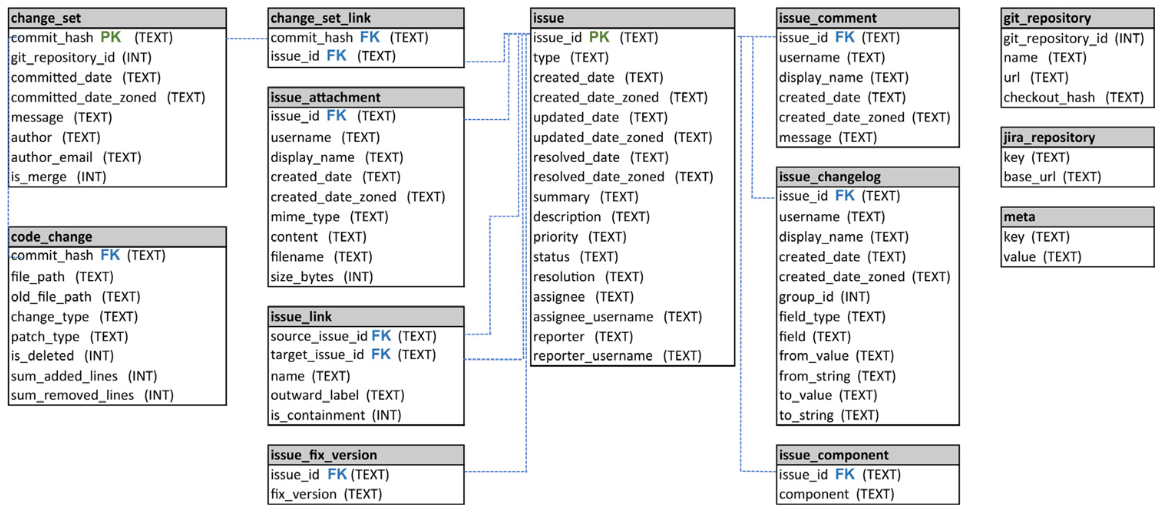
\includegraphics[width=1\textwidth]{pics/seoss/pig.png}
    \caption{Database Schema of the PIG Database \cite{TOMOVA2022108211}}
    \label{fig:SESS}
\end{figure}

Expressions are labeled into two different tags, development and research. Eighty-one queries with a focus on software needs of stakeholders and developers or from typical use cases' queries of issue tracking systems were labeled as 'development,' and 63 queries containing issue tracking systems information or version control systems were labeled as 'research.' Also, 22 records were generated from the content in questions stakeholders asked within the comment sections of issues of type bug, enhancement/improvement, new feature/feature request, and tasks of 33 open-source Apache projects, which were extracted and stored into databases by Rath and Mäder\cite{RATH2019104005}.
In SEOSS-Queries\cite{TOMOVA2022108211} research, they experienced RatSQL and SQLNet methods on the SEOSS dataset and released their evaluation steps. In this research, we will use the same dataset to evaluate state-of-the-art models currently available in the literature and used in SPIDER for this dataset.


% TODO: need more about the Hardness of the SEOSS dataset
% \begin{figure}[H]
%     \centering
%     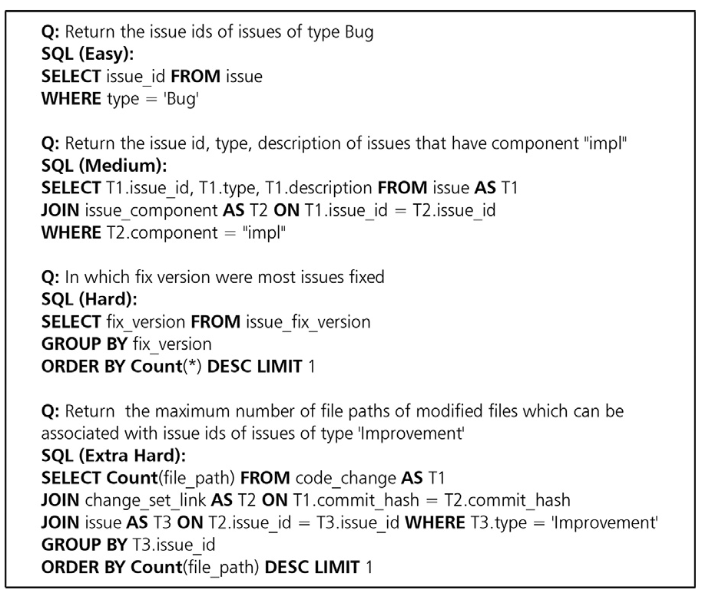
\includegraphics[width=0.8\textwidth]{pics/seoss/seoss.png}
%     \caption{\small Examples of queries with different levels of complexity in SEOSS-Queries \cite{TOMOVA2022108211}}
%     \label{fig:SESS2}
% \end{figure}

\begin{figure}[H]
    \label{fig:SESS2}
    \begin{AIbox}{An example of an extra-hard SEOSS record}
        \vspace{-5px}
        \parbox{1\textwidth}{\scriptsize
        \begin{alltt} \larger
            {\bf Utterance:} \\ 
            Return  the maximum number of file paths of modified files which can be associated with issue ids of issues of type 'Improvement
            \\
            {\bf Query:} \\
            SELECT Count(file\_path) FROM code\_change AS T1 JOIN change\_set\_link AS T2 ON T1.commit\_hash = T2.commit\_hash JOIN issue AS T3 ON T2.issue\_id = T3.issue\_id WHERE T3.type = 'Improvement' GROUP BY T3.issue\_id ORDER BY Count(file\_path) DESC LIMIT 1
        \end{alltt}
        }
        \vspace{-5px}
    \end{AIbox}
    
    \captionsetup{font={scriptsize,color=white}, skip=-20pt}
    \caption{An example of an extra-hard SEOSS record}
\end{figure}

